\section{Seven colour flashing LED module}
\begin{figure}[H]
    \centering
    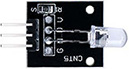
\includegraphics[angle=0, keepaspectratio=true, scale=1, width=200px, height=200px]{images/7_led.jpg}
    %\caption{Caption}
\end{figure}
\subsection*{Description}
This module contains an LED which automatically cycles through seven colours when powered.
\subsection*{Pin mapping}
This pin mapping corresponds to the pins from left to right with the module pins facing towards you.
\begin{table}[H]
    \centering
    \begin{tabular}{|c|c|c|c|c|}
    \hline
    Index &Label &Type &Name &Description\\ \hline
    0 &S &Digital input &D0 &Signal to turn on module\\ \hline
    1 & &Source voltage &$V+$ &Unused\\ \hline
    2 &- &Ground &GND &\\ \hline
    \end{tabular}
    %\caption{Caption}
    %\label{tab:my_label}
\end{table}
\subsection*{Operation}
By setting the digital input pin D0 to high the module can be turned on. Setting D0 to low will turn the module off.
%\subsection*{Code}
%\lstinputlisting[caption=test]{laser.py}